% ----------------------------------------------------------------------------------------------------
\section{Modeling}

% ---------------------------------------------------------------------------------------------------
\subsection{Dataset splitting}
The goal of this study is to predict whether a patient is likely to get a stroke. The target solution 
is the 'stroke' attribute while the data are all the remaining attributes.  

80\% of the dataset is used to train the algorithms and the remaining 20\% are used to test the 
models. K-fold cross-validation is performed to reduce variance and incertainties due to random 
selection of the training and testing datasets. Results are averaged on five folds.

% ---------------------------------------------------------------------------------------------------
\subsection{Class imbalance}
Class imbalance on the target attribute 'stroke' (see section \ref{section_imbalance}) could lead to 
failling model training and predictions. Oversampling might be necessary to counterbalance this 
problem. Figure \ref{distribution_stroke_01} presents the distribution of the attribute 'stroke' as a 
function of 'age', 'avg\_glucose\_level' and 'bmi' (\textit{i.e.} the three numerical values from the 
dataset).

\begin{figure}[H]
\centering
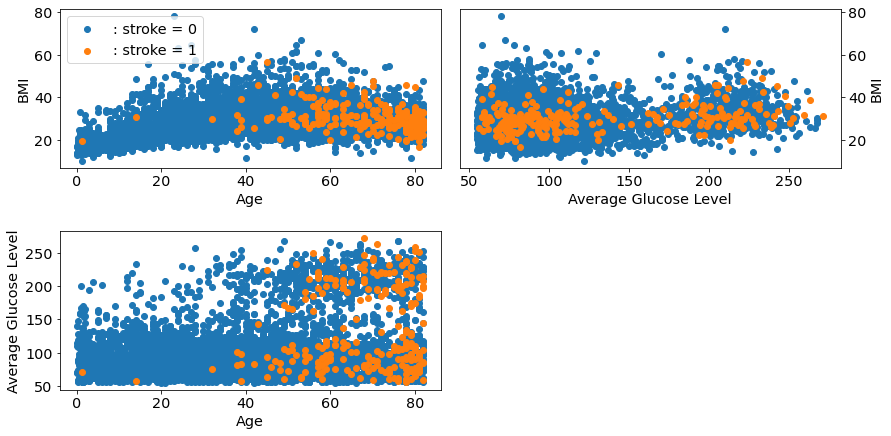
\includegraphics[scale=0.5]{../figures/plot_ageBMIAvgGlucoseLevel_stroke01.png}
\caption{Distribution of the 'stroke' values as a function of attributes 'age', 'bmi' and 'avg\_glucose\_level'.}
\label{distribution_stroke_01}
\end{figure}

Class imbalance is handled using the Synthetic Minority Oversampling Technique (SMOTE). Figures 
\ref{distribution_stroke_01_over} and \ref{figure_Xcorr_over} present the distribution of the 
over-sampled 'stroke' attribute and correlation matrix respectively. As a comparaison with the 
correlation matrix before over-sampling (figure \ref{figure_Xcorr_vector}), only small alteration 
is observed.

\begin{figure}[H]
\centering
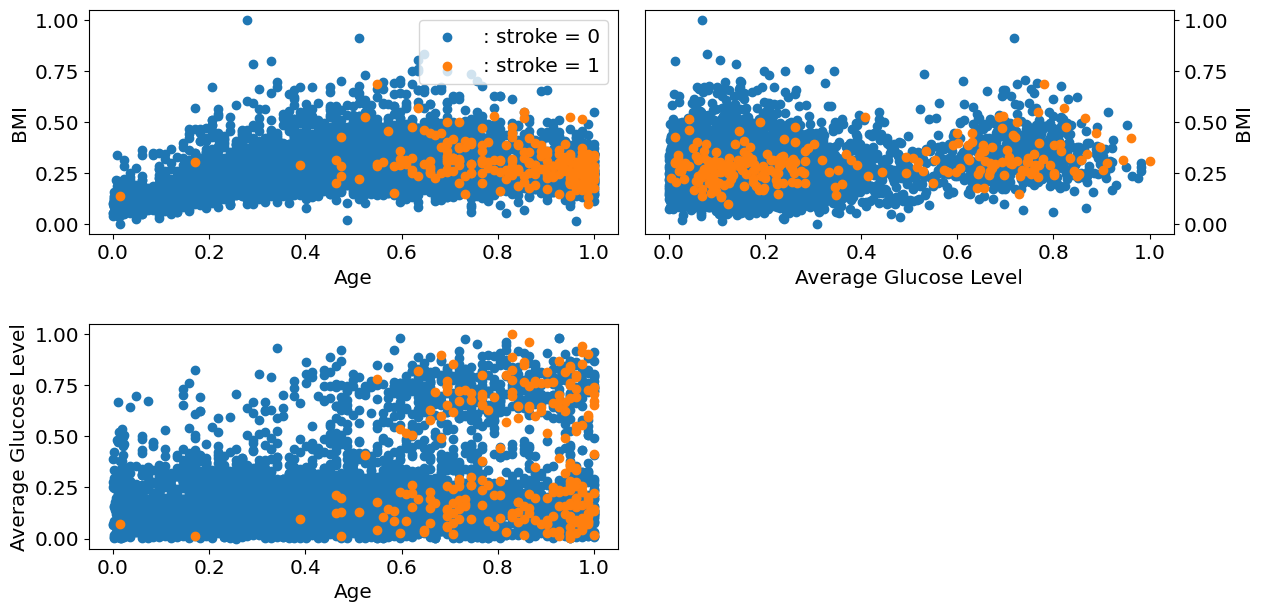
\includegraphics[scale=0.5]{../figures/plot_ageBMIAvgGlucoseLevel_stroke01_over.png}
\caption{Distribution of the 'stroke' values as a function of attributes 'age', 'bmi' and 'avg\_glucose\_level' with oversampling of the minority attributes.}
\label{distribution_stroke_01_over}
\end{figure}

\begin{figure}[H]
\centering
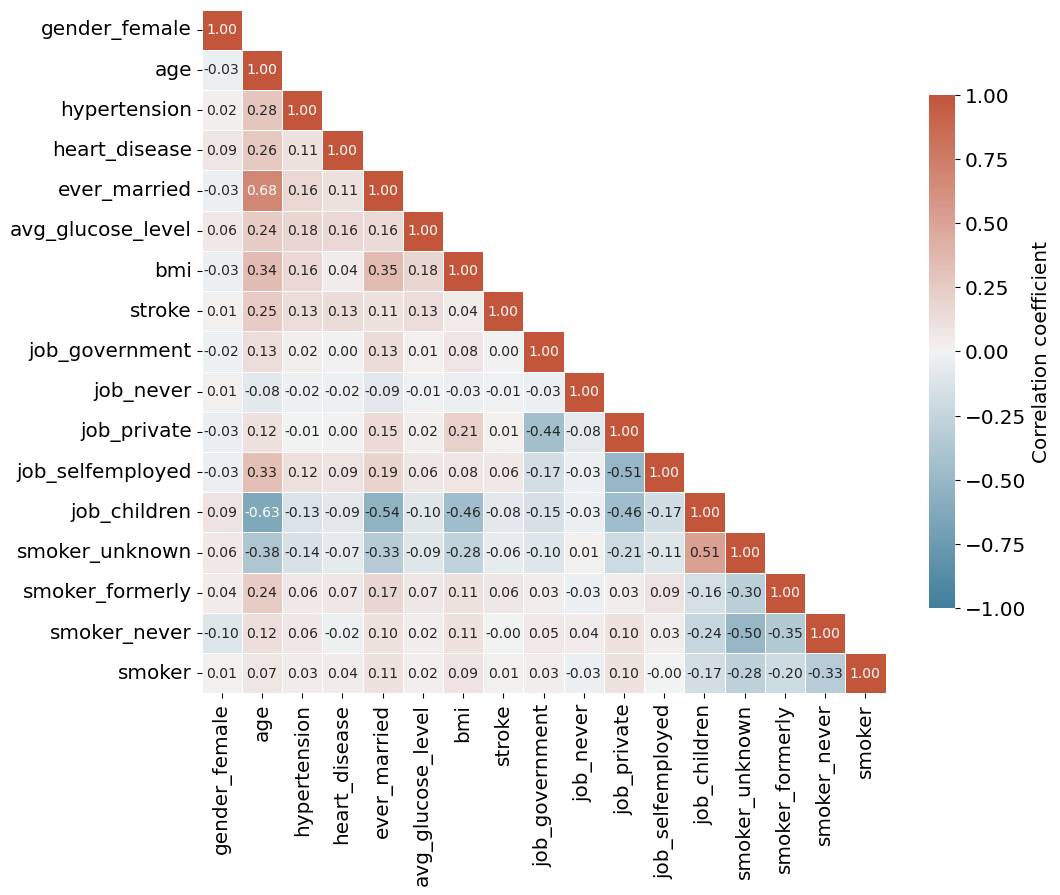
\includegraphics[scale=0.5]{../figures/correlationMatrix_over.png}
\caption{Correlation matrix with oversampling of the minority attributes.}
\label{figure_Xcorr_over}
\end{figure}

\begin{table}[H]
\centering \begin{tabular}{rcc}
\textbf{Attribute} & \textbf{Original dataset} & \textbf{Oversampled dataset}\\\hline\hline
age                & \#           & \# \\
avg\_glucose\_level& \#           & \# \\
bmi                & \#           & \# \\
gender\_female     & 0 (58\%), 1 (41\%) & 0 (60\%), 1 (39\%) \\
hypertension       & 0 (90\%), 1 (9\%)  & 0 (88\%), 1 (12\%) \\
heart\_disease     & 0 (94\%), 1 (5\%)  & 0 (91\%), 1 (9\%) \\
ever\_married      & 0 (34\%), 1 (65\%) & 0 (25\%), 1 (75\%) \\
stroke             & 0 (95\%), 1 (4\%)  & 0 (55\%), 1 (45\%) \\
job\_government    & 0 (87\%), 1 (12\%) & 0 (88\%), 1 (12\%) \\
job\_never         & 0 (99\%), 1 (0\%)  & 0 (99\%), 1 (1\%) \\
job\_private       & 0 (42\%), 1 (57\%) & 0 (40\%), 1 (60\%) \\
job\_selfemployed  & 0 (83\%), 1 (16\%) & 0 (80\%), 1 (20\%) \\
job\_children      & 0 (86\%), 1 (13\%) & 0 (92\%), 1 (8\%) \\
smoker\_unknown    & 0 (69\%), 1 (30\%) & 0 (74\%), 1 (26\%) \\
smoker\_formerly   & 0 (82\%), 1 (17\%) & 0 (77\%), 1 (23\%) \\
smoker\_never      & 0 (62\%), 1 (37\%) & 0 (63\%), 1 (37\%) \\
smoker             & 0 (84\%), 1 (15\%) & 0 (84\%), 1 (16\%) \\
\end{tabular}
\caption{Table of attributes of the datasets with their possible values and corresponding frequency. The original dataset has 5107 entries and the oversampled dataset has 8802 entries.}
\label{}
\end{table}

% ----------------------------------------------------------------------------------------------------
\subsection{Model training and evaluation using classification algorithms}

Classification algorithms are applied to the dataset to predict the value of the 'stroke'. The 
classifiers used are Logistic Regression, Random Forest and Multi-layer Perceptron. 
Results for each of the algorithms are presented below.\\

Several evaluation metrics are computed for each modeling and for the dataset with or without 
oversampling :
\begin{itemize}
 \item \textbf{Recall} $\in [0;1]$ : measures how much of the positive data are well recovered from the dataset.
 \item \textbf{Precision} $\in [0;1]$ : measures how much of the positive prediction are correct, 
 \item \textbf{F1-score} $\in [0;1]$ : informs on the performance of the prediction. Maximizing F1-score implies maximizing both the recall and precision.
 \item \textbf{Accuracy} $\in [0;1]$ : informs on the ability of the model to make a correct prediction.
\end{itemize} 

% ----------------------------------------------------------------------------------------------------
\subsubsection{Logistic Regression}
Logistic regression algorithm from the Python \texttt{sklearn} library search for a model that 
minimizes the residual squared sum between the observations and the model using linear 
approximation.\\

Metrics presented in Table \ref{table_LR} and figure \ref{figure_metrics_LR} show that oversampling 
helps improve the identification of the positive target (higher values of recall). Although some 
improvement is observed, applying oversampling to the data does not improve the performance of the 
prediction (\textit{i.e.} precision and F1-score values remain small). Results are consistent along 
each set of five runs. 

The process time on a regular laptop is 0.074~s for the original dataset sampling and 0.234~s for the 
oversampled dataset.

\begin{table}[H]
\centering \begin{tabular}{c|ccccc}
& \textbf{Run} & \textbf{Recall} & \textbf{Precision} & \textbf{F1-score} & \textbf{Accuracy}\\\hline \hline
\parbox[t]{2mm}{\multirow{5}{*}{\rotatebox[origin=c]{90}{No SMOTE}}} 
& 1 & 0.0  &  0.0 & 0.0 & 0.756 \\
& 2 & 0.0  & 0.0  & 0.0  & 0.753 \\
& 3 & 0.0  & 0.0  & 0.0  & 0.727 \\
& 4 & 0.0  & 0.0  & 0.0  & 0.743 \\
& 5 & 0.0  & 0.0  & 0.0  & 0.776 \\ \hline
\parbox[t]{2mm}{\multirow{5}{*}{\rotatebox[origin=c]{90}{SMOTE}}} 
& 1 & 0.74 & 0.136 & 0.229 & 0.756 \\
& 2 & 0.72 & 0.131 & 0.222 & 0.753 \\
& 3 & 0.78 & 0.137 & 0.218 & 0.726 \\
& 4 & 0.78 & 0.134 & 0.229 & 0.743 \\
& 5 & 0.76 & 0.146 & 0.244 & 0.775 \\
\end{tabular}
\caption{Recall, precision, F1-score and accuracy metrics computed for five folds using the original dataset sampling (no SMOTE) and the oversampled dataset (SMOTE) and logistic regression algorithm.}
\label{table_LR}
\end{table}

\begin{figure}[H]
\centering
  \subfloat[\centering No SMOTE]
   {{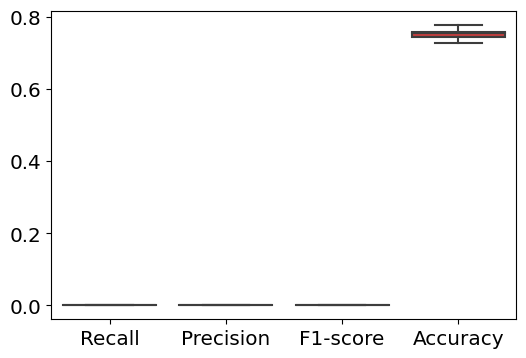
\includegraphics[scale=0.5]{../figures/boxplot_LogisticRegression_smote0.png}}}
  \qquad
  \subfloat[\centering SMOTE]
  {{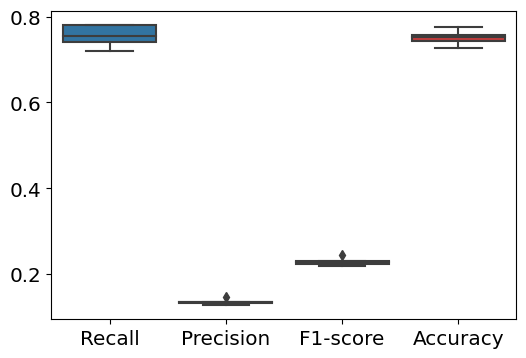
\includegraphics[scale=0.5]{../figures/boxplot_LogisticRegression_smote1.png}}}
\caption{Boxplot representation of the recall, precision, F1-score and accuracy metrics computed for five folds using the original dataset sampling (a) and the oversampled dataset (b) and logistic regression algorithm.}
\label{figure_metrics_LR}
\end{figure}

% ----------------------------------------------------------------------------------------------------
%\subsubsection{Decision Tree}
%Decision tree algorithm from the Python \texttt{sklearn} library search for a best-fitting model 
%using a decision tree structure. 
%
%
%%\red{process time: DecisionTreeClassifier 0 : 0.0132 ; DecisionTreeClassifier 1 : 0.0558}
%
%\begin{table}[H]
%\centering \begin{tabular}{c|ccccc}
%& \textbf{Run} & \textbf{Recall} & \textbf{Precision} & \textbf{F1-score} & \textbf{Accuracy}\\\hline \hline
%\parbox[t]{2mm}{\multirow{5}{*}{\rotatebox[origin=c]{90}{No SMOTE}}} 
%& 1 & 0.16  & 0.136 & 0.147 & 0.874 \\
%& 2 & 0.22  & 0.194 & 0.207 & 0.835 \\
%& 3 & 0.14  & 0.097 & 0.114 & 0.858 \\
%& 4 & 0.16  & 0.154 & 0.157 & 0.873 \\
%& 5 & 0.14  & 0.115 & 0.127 & 0.858 \\ \hline
%\parbox[t]{2mm}{\multirow{5}{*}{\rotatebox[origin=c]{90}{SMOTE}}} 
%& 1 & 0.200 & 0.101 & 0.134 & 0.874 \\
%& 2 & 0.320 & 0.106 & 0.159 & 0.835 \\
%& 3 & 0.220 & 0.094 & 0.132 & 0.858 \\
%& 4 & 0.260 & 0.122 & 0.167 & 0.873 \\
%& 5 & 0.245 & 0.099 & 0.141 & 0.857 \\
%\end{tabular}
%\caption{Recall, precision, F1-score and accuracy metrics computed for five folds using the original dataset sampling (no SMOTE) and the oversampled dataset (SMOTE) and decision tree algorithm.}
%\label{table_DT}
%\end{table}

%\begin{figure}[H]
%\centering
%  \subfloat[\centering No SMOTE]
%   {{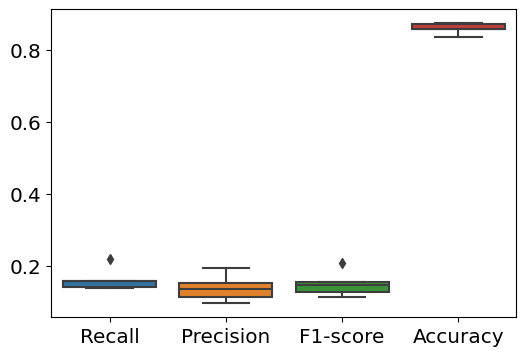
\includegraphics[scale=0.5]{../figures/boxplot_DecisionTreeClassifier_smote0.png}}}
%  \qquad
%  \subfloat[\centering SMOTE]
%   {{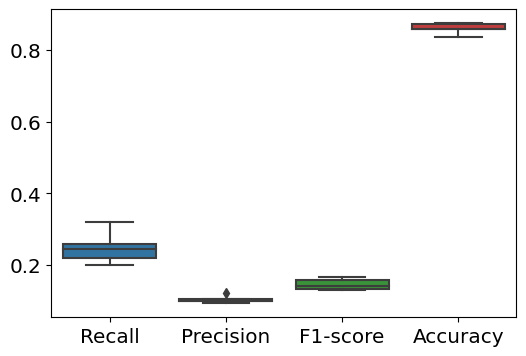
\includegraphics[scale=0.5]{../figures/boxplot_DecisionTreeClassifier_smote1.png}}}
%\caption{Boxplot representation of the recall, precision, F1-score and accuracy metrics computed for five folds using the original dataset sampling (a) and the oversampled dataset (b) and decision tree algorithm.}
%\label{figure_metrics_DT}
%\end{figure}

% ----------------------------------------------------------------------------------------------------
\subsubsection{Random forest}
Random Forest algorithm from the Python \texttt{sklearn} library search for a best-fitting model 
using decision tree classifiers on sub-samples of the dataset.\\ 

Metrics presented in Table \ref{table_RF} and figure \ref{figure_metrics_RF} show that oversampling 
slightly improves the identification of the positive target (higher values of recall). Although some 
improvement is observed, applying oversampling to the data does not improve the performance of the 
models (\textit{i.e.} recall, precision and F1-score values remain small). Results are consistent 
along each set of five runs. 

The process time on a regular laptop is 0.593~s for the original dataset sampling and 1.069~s for the 
oversampled dataset.

\begin{table}[H]
\centering \begin{tabular}{c|ccccc}
& \textbf{Run} & \textbf{Recall} & \textbf{Precision} & \textbf{F1-score} & \textbf{Accuracy}\\\hline \hline
\parbox[t]{2mm}{\multirow{5}{*}{\rotatebox[origin=c]{90}{No SMOTE}}} 
& 1 & 0.0   & 0.0  & 0.0  & 0.867 \\
& 2 & 0.02  & 0.33 & 0.04 & 0.883 \\
& 3 & 0.0   & 0.0  & 0.0  & 0.852 \\
& 4 & 0.0   & 0.0  & 0.0  & 0.863 \\
& 5 & 0.02  & 0.33 & 0.04 & 0.867 \\ \hline
\parbox[t]{2mm}{\multirow{5}{*}{\rotatebox[origin=c]{90}{SMOTE}}} 
& 1 & 0.240 & 0.109 & 0.150 & 0.867 \\
& 2 & 0.300 & 0.150 & 0.200 & 0.883 \\
& 3 & 0.320 & 0.120 & 0.174 & 0.852 \\
& 4 & 0.380 & 0.148 & 0.213 & 0.863 \\
& 5 & 0.265 & 0.115 & 0.160 & 0.867 \\
\end{tabular}
\caption{Recall, precision, F1-score and accuracy metrics computed for five folds using the original dataset sampling (no SMOTE) and the oversampled dataset (SMOTE) and random forest algorithm.}
\label{table_RF}
\end{table}


\begin{figure}[H]
\centering
  \subfloat[\centering No SMOTE]
   {{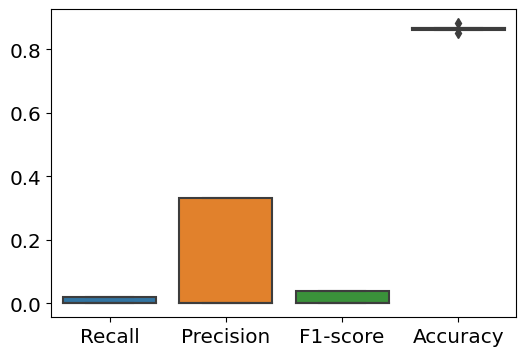
\includegraphics[scale=0.5]{../figures/boxplot_RandomForestClassifier_smote0.png}}}
  \qquad
  \subfloat[\centering SMOTE]
  {{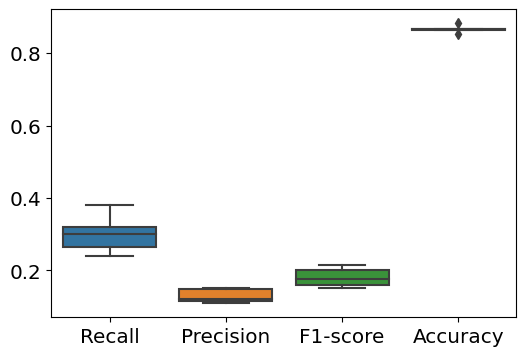
\includegraphics[scale=0.5]{../figures/boxplot_RandomForestClassifier_smote1.png}}}
\caption{Boxplot representation of the recall, precision, F1-score and accuracy metrics computed for five folds using the original dataset sampling (a) and the oversampled dataset (b) and random forest algorithm.}
\label{figure_metrics_RF}
\end{figure}

% ----------------------------------------------------------------------------------------------------
\subsubsection{Multi-layer Perceptron}
Multi-layer Perceptron algorithm from the Python \texttt{sklearn} library search for a best-fitting 
model using non-linear neural networks.\\

Metrics presented in Table \ref{table_MLP} and figure \ref{figure_metrics_MLP} show that oversampling improves the identification of the positive target (higher values of recall). Although some 
improvement is observed, applying oversampling to the data does not improve the performance of the 
models (\textit{i.e.} recall, precision and F1-score values remain small). Results are consistent 
along each set of five runs. 

The process time on a regular laptop is 5.871~s for the original dataset sampling and 39.602~s for 
the oversampled dataset.

\begin{table}[H]
\centering \begin{tabular}{c|ccccc}
& \textbf{Run} & \textbf{Recall} & \textbf{Precision} & \textbf{F1-score} & \textbf{Accuracy}\\\hline \hline
\parbox[t]{2mm}{\multirow{5}{*}{\rotatebox[origin=c]{90}{No SMOTE}}} 
& 1 & 0.0   & 0.0  & 0.0  & 0.795 \\
& 2 & 0.0   & 0.0  & 0.0  & 0.822 \\
& 3 & 0.0   & 0.0  & 0.0  & 0.777 \\
& 4 & 0.0   & 0.0  & 0.0  & 0.777 \\
& 5 & 0.02  & 0.5  & 0.04 & 0.828 \\ \hline
\parbox[t]{2mm}{\multirow{5}{*}{\rotatebox[origin=c]{90}{SMOTE}}} 
& 1 & 0.460 & 0.112 & 0.180 & 0.795 \\
& 2 & 0.460 & 0.129 & 0.202 & 0.882 \\
& 3 & 0.440 & 0.099 & 0.162 & 0.777 \\
& 4 & 0.620 & 0.129 & 0.214 & 0.777 \\
& 5 & 0.388 & 0.115 & 0.178 & 0.828 \\
\end{tabular}
\caption{Recall, precision, F1-score and accuracy metrics computed for five folds using the original dataset sampling (no SMOTE) and the oversampled dataset (SMOTE) and multi-layer perceptron algorithm.}
\label{table_MLP}
\end{table}


\begin{figure}[H]
\centering
  \subfloat[\centering No SMOTE]
   {{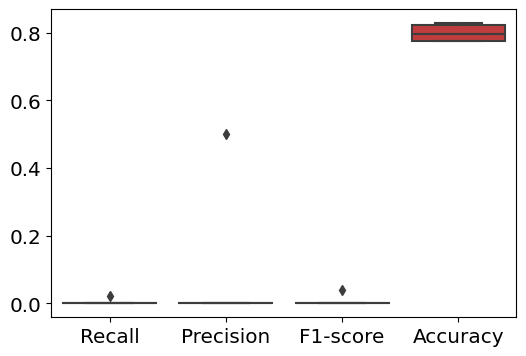
\includegraphics[scale=0.5]{../figures/boxplot_MLPClassifier_smote0.png}}}
  \qquad
  \subfloat[\centering SMOTE]
  {{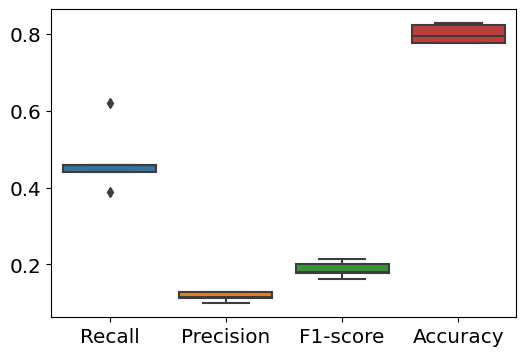
\includegraphics[scale=0.5]{../figures/boxplot_MLPClassifier_smote1.png}}}
\caption{Boxplot representation of the recall, precision, F1-score and accuracy metrics computed for five folds using the original dataset sampling (a) and the oversampled dataset (b) and multi-layer perceptron algorithm.}
\label{figure_metrics_MLP}
\end{figure}

